%
% Annual Cognitive Science Conference
% Sample LaTeX Paper -- Proceedings Format
%

% Original : Ashwin Ram (ashwin@cc.gatech.edu)       04/01/1994
% Modified : Johanna Moore (jmoore@cs.pitt.edu)      03/17/1995
% Modified : David Noelle (noelle@ucsd.edu)          03/15/1996
% Modified : Pat Langley (langley@cs.stanford.edu)   01/26/1997
% Latex2e corrections by Ramin Charles Nakisa        01/28/1997
% Modified : Tina Eliassi-Rad (eliassi@cs.wisc.edu)  01/31/1998
% Modified : Trisha Yannuzzi (trisha@ircs.upenn.edu) 12/28/1999 (in process)
% Modified : Mary Ellen Foster (M.E.Foster@ed.ac.uk) 12/11/2000
% Modified : Ken Forbus                              01/23/2004
% Modified : Eli M. Silk (esilk@pitt.edu)            05/24/2005
% Modified : Niels Taatgen (taatgen@cmu.edu)         10/24/2006
% Modified : David Noelle (dnoelle@ucmerced.edu)     11/19/2014

%% Change "letterpaper" in the following line to "a4paper" if you must.

\documentclass[10pt,letterpaper]{article}


\usepackage{cogsci}
\usepackage{pslatex}
\usepackage{apacite}
\usepackage{graphicx}

% for inline comments
\usepackage{color}
\definecolor{Red}{RGB}{255,0,0}
\newcommand{\mcf}[1]{\textcolor{Red}{[mcf: #1]}}

\title{Inferring Generic Meaning From Pragmatic Reference Failure}

\author{{\large \bf Phil Crone} \\
	\texttt{pcrone@stanford.edu}\\
  Department of Linguistics \\
  Stanford University
  \And {\large \bf Michael C. Frank} \\
  \texttt{mcfrank@stanford.edu}\\
  Department of Psychology \\
  Stanford University}

\begin{document}

\maketitle

\begin{abstract}
Generic sentences (e.g., ``birds lay eggs'') express generalizations about kinds, rather than facts about specific individuals or sets of individuals (e.g., ``all birds lay eggs''). Although generics are an important method of transmitting cultural knowledge, there is no unique linguistic marker of genericity, making the identification of generics a challenge. Here we pursue the hypothesis that generic meanings arise as a result of the failure to ground expressions as referring to particular entities or events. In four experiments, we show that whether particular morphosyntactic and contextual factors support generic or non-generic interpretations for sentences can be tied to whether these factors allow for referential grounding of linguistic expressions or not.

\textbf{Keywords:} Psycholinguistics; pragmatics; generics.
\end{abstract}


\section{Introduction}

Generic sentences express generalizations about kinds rather than individuals and are an important route for the transmission of cultural knowledge \cite{gelman2003}. For example, the sentence ``birds fly'' expresses a general property of the kind \textit{bird}, whereas ``all birds fly'' means that every member of the set flies. A key difference between generic and non-generic statements is that generics allow for exceptions: ``birds fly'' is true despite the fact that some birds do not fly, while ``all birds fly'' is false, because, e.g., emus do not fly \cite{Prasada:2000}.

Generics are not consistently marked by any particular lexical, morphological, or syntactic convention, so how do we know that a sentence is generic? Prior work suggest that we use at least three types of cues to guide the interpretation of sentences as generic or non-generic: morphosyntactic features, pragmatic cues, and world knowledge. In English, the subject noun phase (NP) of a generic sentence is often a bare plural (``birds fly''), but it can also be an indefinite singular (``a bird has feathers'') or definite singular (``the bird is a warm-blooded animal''). In contrast, definite plural NPs (``the birds have beaks'') are generally thought to force non-generic interpretations. Tense and aspect also cue whether a sentence is interpreted generically; simple present tense (``birds fly'') is typically more generic than e.g., present progressive (``birds are flying overhead'') or past (``birds flew past my window'') \cite{Carlson:1977,Krifka:1995,Lyons:1977}.

Pragmatics and world knowledge are also argued to influence a sentence's interpretation as generic or non-generic. For example, if a unique bird is present in the context of an utterance of a sentence with the subject NP ``the bird,'' this NP is likely to be interpreted as referring to the bird in context, giving rise to a non-generic interpretation. And if world knowledge about properties shared by members of a kind influences the interpretation of potentially generic sentences. The sentence ``a bird does not fly'' is interpreted as being about some particular bird (e.g., a penguin), given world knowledge that, in general, birds fly.

Previous experimental work has confirmed the influence of these three factors---NP type, pragmatic context, and world knowledge---on the interpretation of sentences as generic. Adults can also use the definiteness of subject NPs, as well as tense and aspect, to identify generics, and prefer generic interpretations when the subject NP has no available referent in context \cite{Gelman:2003,Cimpian:2011}. By age 3, children are less likely to assign a generic interpretation to a sentence when its subject NP has a possible referent in the preceding linguistic context and can also use knowledge about the generalizability of properties to kinds in identifying generics \cite{Cimpian:2008}.

% \footnote{As in previous work, we focus on generics that describe kinds (e.g., ``Birds lay eggs.'') rather than habitual generics (e.g., ``John walks to school.'').}

In the current paper, we synthesize these previous findings under a single explanation, arguing that generic interpretations are driven by a failure to find reference for entities or events described by the sentence in question. We hypothesize that listeners consider two possible interpretations of generic statements: either there is a particular entity or set of entities that the speaker is trying to inform them about, or else the speaker is trying to be informative about a kind.

This hypothesis---which we refer to as the ``pragmatic reference failure'' hypothesis---is based on the finding that the referential status of definite NPs affects judgements of genericity \cite{Gelman:2003}. It also provides a candidate explanation for morphosyntactic effects. Like referential context, features like tense and definiteness influence the probability that a particular speaker was referring to a specific entity. ``A dog had legs'' is an odd statement, but it seems to play the pragmatic role of introducing a dog into the discourse and predicating a feature to it. In contrast, ``A dog has legs'' could in principle introduce an entity that is currently present in the context, but this interpretation is unlikely because A) there probably isn't a dog present, and B) if there were, it would be in the common ground and hence wouldn't require an indefinite article.

In our current nvestigation, we build on empirical work described by \citeA{Gelman:2003} and \citeA{Cimpian:2008} by assessing the impact of morphosyntactic and contextual factors on adults' judgments about genericity across a wide variety of sentences. Most previous work on the identification of generics has focused on children's abilities, perhaps stemming in part from an assumption that children face challenges in identifying generics that are less relevant for adults. However, research on the probabilistic nature of language comprehension suggests that adults face a similar problem \cite{Levy:2008,Frank:2012}. In the case of identifying generics, we can take adults to reason about the likelihood that an utterance is generic given morphosyntactic features of the sentence, features of the context, and the their own world knowledge. Second, we collect naturalistic examples of generic and non-generic sentences generated by study participants, allowing us to consider a realistic representation of genericity in natural language.\mcf{would like to cite degen's scalar corpus paper here somewhere.}

The plan of the paper is as follows. We gather a corpus of generic and non-generic sentences from experimental participants' productions and then elicit independent ratings of genericity for these sentences, using this paradigm to examine the role of morphosyntactic information of a sentence's subject NP in determining genericity (Experiment 1). We next consider several machine learning techniques for classifying sentences as generic or not, finding that just two factors, definiteness of the subject NP and tense, prove extremely successful in classifying sentences (Experiment 2). Next, we validate the importance of tense for generic interpretation with human subjects (Experiment 3). Finally, we manipulate contextual information to show that the availability of a referent for the subject NP of a sentence influences interpretation (Experiment 4). Taken together, the results of these experiments show that judgments of whether a sentence is generic or non-generic can largely be explained by considering whether the sentence can be referentially grounded in some specific entity or event.

\section{Experiment 1}

As discussed above, it has been argued that the number and definiteness of a sentence's subject NP influence its interpretation as generic or non-generic \cite{Carlson:1977,Krifka:1995,Lyons:1977}. Previous work investigating these cues to genericity have fixed the number of the subject NP as either singular \cite{Cimpian:2011} or plural \cite{Gelman:2003} and only manipulated definiteness. In Experiment 1, we considered the effects of number, definiteness, and their interaction on the interpretation of generics. Participants performed a sentence completion task in which the subject NP was provided. They then indicated whether the sentences they produced were about specific individuals or kinds. In this experiment, we were interested in participants' judgements of their own intentions in producing the sentences; in Experiment 2, we elicit independent ratings of these same sentences.

\subsection{Method}

\subsubsection{Participants}

We recruited 100 participants to participate through Amazon's Mechanical Turk website. We restricted participants to individuals within the United States and paid them 50 cents to complete the study. The study took approximately 14 minutes to complete. We excluded 4 participants for indicating that their native language was not English.

\subsubsection{Stimuli}

Forty-eight nouns, split evenly between animates and inanimates, were chosen to use as the bases for subject NPs. For each participant, each noun was randomly assigned morphosyntactic features using a \(2 \times 2\) factorial design crossing number (singular, plural) with definiteness (definite, indefinite). Half of nouns assigned to each factorial point were animate and half were inanimate. Full NPs were created from the base noun, and number and definiteness features. For example, if the noun ``panda'' were assigned values \textit{plural} and \textit{definite}, the full NP would be ``the pandas.''

In the first part of the experiment, participants saw a sequence of these NPs followed by a text box. They were instructed to ``write a sentence starting with the phrase below.'' In the second part of the experiment, participants were shown the sentences they had written in the first part of the experiment. They viewed one sentence at a time and were asked whether the sentence was about a specific \textit{noun} (for singular NPs), a specific group of \textit{nouns} (for plural NPs), or about \textit{nouns} in general. Participants indicated their response using a 5-point Likert scale with the following values: ``Definitely about a specific \textit{noun}/group of \textit{nouns} (=1),'' ``Probably about a specific \textit{noun}/group of \textit{nouns},'' ``Not sure,'' ``Probably about \textit{nouns} in general,'' ``Definitely about \textit{nouns} in general (=5).''

\subsubsection{Procedure}

We first presented participants with four example NPs. After providing a sentence completion for each example item, participants were shown an example sentence completion for the given NP. These sentences were constructed to favor non-generic interpretations for all NP types. After seeing the examples, participants were informed that they would not receive any feedback for the rest of the experiment.

Participants then began the first part of the experiment. All forty-eight subject NPs were presented in pseudorandom order, counterbalanced so that no two consecutive NPs matched in both number and definiteness. Participants had to provide a sentence completion at least six characters in length for each item. After completing part 1, participants entered the second part of the experiment and were informed that they would be evaluating the sentences they had produced in part 1 in the manner described above. Sentences were again presented in a pseudorandom order counterbalanced so that no two consecutive NPs matched in both number and definiteness. After judging all forty-eight sentences, participants were required to report their native language. We measured reaction times for each item, measured from the time the item was presented until the time a response was submitted. In analyzing results from the second part of the experiment, we excluded responses whose reaction times were greater than 2 standard deviations from the mean.

% \subsubsection{Data Analysis}

\begin{table*}
\begin{center}
\caption{Example Productions from Experiment 1. Generic sentences received ratings of 5; non-generics received ratings of 1.}
\label{tab:ex}
\vskip 0.12in
\begin{tabular}{cccc}
\hline
Definiteness    &  Number & Genericity & Examples \\
\hline
Indefinite        &   Singular & Generic & ``A cow eats grass.'', ``A bicycle is a convenient form of transportation.''\\
Indefinite  &   Singular & Non-generic & ``A dog is sleeping on the porch.'', ``A light bulb was dropped and exploded.''\\
Indefinite           &   Plural & Generic & ``Gorillas are primates.'', ``Towels are useful after showering.''\\
Indefinite         &   Plural  & Non-generic & ``Cats are circling the fishtank.'', ``Kites were flying at the beach.''\\
Definite        &   Singular & Generic & ``The camel uses his humps to conserve water.'', ``The clock tells time.''  \\
Definite  &   Singular & Non-generic & ``The bear is moving closer to us.'', ``The bed is unmade.''\\
Definite           &   Plural & Generic & ``The kangaroos carry babies in pouches.'', ``The trumpets are loud.'' \\
Definite         &   Plural & Non-generic & ``The rabbits are digging holes in the yard.'', ``The couches were dusty and old.''\\
\hline
\end{tabular}
\end{center}
\end{table*}

\subsection{Results and Discussion}

We found that both definiteness and number affected mean genericity ratings (Figure \ref{fig:e1}). Sentences with definite subject NPs tended to be rated as less generic, while those with indefinite subjects---especially ``bare plural'' subjects---tended to be rated as more generic (see Table \ref{tab:ex} for examples).

\begin{figure}[t]
\centering
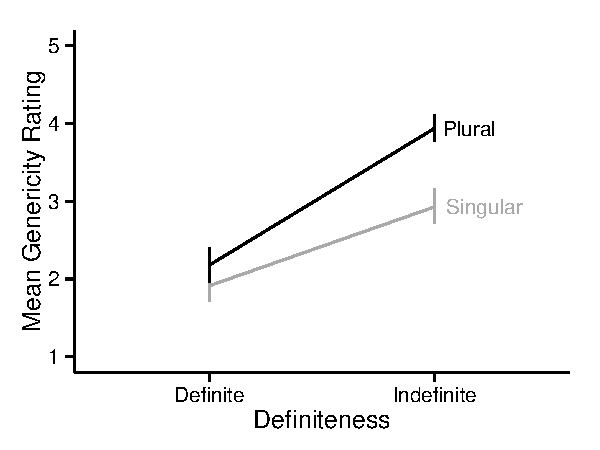
\includegraphics[width=.8\linewidth]{figures/e1.pdf}
\caption{\label{fig:e1} Mean genericity ratings in Experiment 1 by definiteness and number. Error bars show 95\% confidence intervals.}
\end{figure}

To analyze the results, we fit a linear mixed-effects model to predict participants' genericity ratings. We examined the interaction between animacy, definiteness, and number of subject NPs.\footnote{Mixed-effects models were fit in R v. 3.1.2 using the lme4 package. The model specification was as follows: \texttt{response} \(\sim\) \texttt{animacy * definiteness * number + (animacy + definiteness + number | WorkerId) + (definiteness + number | subject noun)}. We calculated \(p\) values by treating the \(t\) statistic as if it were a \(z\) statistic \cite{Barr:2013}.} The model shows main effects of animacy, definiteness, and number. Sentences with indefinite NP subjects were rated significantly more generic (\(\beta = 1.75,~t = 14.17,~p < 0.01\)). Sentences with singular NP subjects (\(\beta = -0.30,~t = -3.45,~p < 0.01\)) and inanimate subjects (\(\beta = -0.50,~t = -5.73,~p < 0.01\)), were rated less generic. In addition, the model revealed an interaction effect between definiteness and number such that indefinite singulars were rated significantly less generic (\(\beta = -1.02,~t = -9.91,~p < 0.01\)). Finally, there was a significant three-way interaction such that inanimate, indefinite singulars were rated significantly more generic (\(\beta = 0.54,~t = 3.67,~p < 0.01\)).

The results are consistent with previous findings that indefinite singulars and bare plurals facilitate generic interpretations compared to definite singulars and definite plurals, respectively \cite{Cimpian:2011, Gelman:2003}. Indeed, we found number to have the largest effect size of all predictors (\(\beta = 1.75\)). This result is straightforwardly interpretable in terms of the general hypothesis that generic interpretation arises from reference failure. Since the definite determiner \textit{the}, unlike indefinite determiners, is generally taken to presuppose the existence of a unique, salient entity, it follows that definite subject NPs are more likely to refer to some particular entity. Therefore, sentences with such subjects are less likely to have an intended generic interpretation.

These results also show that plurality is independently associated with genericity, which has not been previously acknowledged. However, the effect size associated with number was relatively small (\(\beta = -0.30\)). The interaction between definiteness and plurality reveals a superadditive effect by which indefinite, bare plurals were rated more generic than would be predicted by the main effects of indefinitenes and plurality. This is unsurprising, as bare plurals are often taken to be the canonical subject type for English generics. The effect of animacy is also consistent with previous findings that both children and adults produce more generic statements when describing animals than when describing artifacts \cite{Brandone:2009}.

One unexpected finding is sentences produced with definite plural subjects were rated more generic overall than definite singulars, despite the general view that definite singulars, but not definite plurals, allow for generic interpretations in English. This result forced us consider whether our methodology measured some property other than genericity. However, inspection of definite plurals that received high genericity ratings suggested that these ratings were at least \emph{prima facie} appropriate (Table \ref{tab:ex}). Overall, ratings for sentences with definite plural subjects were still quite low.

\section{Experiment 2}

The results of Experiment 1 appear to show that multiple factors help determine the genericity of sentences and that the definiteness of the subject NP plays a particularly large role in determining a sentence's interpretation. However, there are a number of factors that have previously been acknowledged to influence interpretations of genericity, such as tense and aspect, that were not manipulated in Experiment 1, and may have co-varied with condition in participants' productions. In addition, since the same subjects produced and interpreted the same set of sentences, their responses in part 2 might have reflected intuitions that were not directly communicated in the linguistic forms of the sentences. To address these issues, we collected independent judgments about the sentences produced in Experiment 1 from a new set of participants and used these to explore factors that influence generic interpretation more broadly.

\subsection{Method}

\subsubsection{Participants}

We recruited two sets of participants. For each set, recruitment details were as above, except that the experiment took approximately 5 minutes and participants were paid 50 cents each. We recruited 94 participants for the first set and \(n\) participants from the second set. We excluded from the analysis 6 participants from the first set and \(m\) participants from the second set who indicated that they were non-native English speakers.\mcf{FIXME}

\subsubsection{Stimuli}

For both sets of participants, stimuli consisted of sentences produced by participants in Experiment 1. Participants responded to these sentences via a binary forced-choice task. For a sentence whose subject NP used a base noun \textit{noun}, participants were asked to indicate whether this sentence was about \textit{nouns} or about a specific \textit{noun} (singular subject NP) or a specific group of \textit{nouns} (plural subject NP). All sentences produced in Experiment 1 were judged by at least one participant from the first set of participants in Experiment 2. One quarter of the sentences produced in Experiment 1 were rated a second time by at least one participant from the second set of participants in Experiment 2.

\subsubsection{Procedure}

Participants were instructed that they would be viewing a sequence of 50 sentences that had been produced by other Mechanical Turk workers. Participants began by judging 4 warm-up sentences constructed by the experimenters for which the participants received feedback. After these 4 sentences, participants did not receive any additional feedback. The remaining sentences were presented in random order.

\subsection{Results and Discussion}

The responses in Experiment 2 from the first set of participants were broadly similar to those in Experiment 1 (Figure \ref{fig:e2}). Once again, sentences with definite subject NPs were less likely to be rated generic, whereas those with bare plural subject NPs were highly likely to be rated generic. We first analyzed the results from the first set of participants in Experiment 2 using a logistic mixed-effects model, which predicted whether a sentence would be rated generic or not from the interaction between definiteness, number, and animacy of the subject NP.\footnote{The model specification was as in Experiment 1, except that we used a logistic---rather than a linear---mixed-effects model.} The model identified significant main effects of definiteness such that sentences with indefinite subject NPs were more likely to be rated generic (\(\beta = 3.29, z = 14.41, p < 0.001\)) and animacy such that sentences with inanimate subjects were less likely to be rated generic (\(\beta = -1.29, z = -3.33, p < 0.001\)). There were also significant interactions between animacy and definiteness such that sentences with inanimate, indefinite subjects were more likely to be rated generic (\(\beta = 0.86, z = 2.52, p < 0.05\)) and between definiteness and number such that sentences with indefinite, singular subjects were less likely to be rated generic (\(\beta = -1.84, z = -7.59, p < 0.001\)). Note that in contrast to Experiment 1, sentences with definite plural subjects were not found to be judged generic more often than those with definite singular subjects.

\begin{figure}[t]
\centering
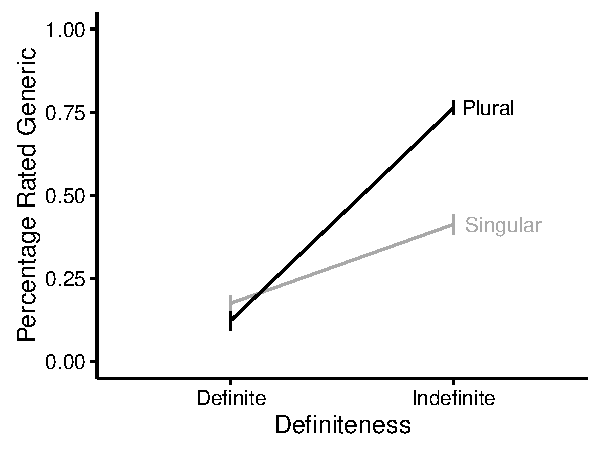
\includegraphics[width=.8\linewidth]{figures/e2-2016.pdf}
\caption{\label{fig:e2} Percentage of sentences rated generic in Experiment 2 by definiteness and number. Error bars show 95\% confidence intervals.}
\end{figure}

\section{Genericity Classification}
To probe other factors that influence judgments of genericity, we extracted additional linguistic information from the sentences tested. We first used the Stanford part-of-speech (POS) tagger \cite{Toutanova:2003} to obtain POS tags for all sentences judged in this experiment. Using these POS tags, we automatically extracted the following features for each sentence: tense, aspect, presence of main verb \textit{be} or \textit{have}, and presence of a modal. We also extract total sentence length minus the length of the subject NP for each sentence.

We next split the data from the first set of participants into training and test sets, with the training set consisting of 75\% of the sentences judgment by the first set of participants in Experiment 2. We next trained a variety of classification models on this training set, including generalized linear models, basic decision trees, boosted trees, and random forests. All model parameters were optimized using 10-fold cross-validation. The resulting models were then evaluated on the 25\% held-out test set. All classification techniques achieved accuracy on the test set of 86\%-88\%. The most straightforwardly interpretable of these methods is the basic decision tree pruned to have three terminal nodes (Figure \ref{fig:e2-tree}).\footnote{An initial decision tree was fit using the \texttt{tree} package with the specification \texttt{response} \(\sim\) \texttt{number + definiteness + animacy + tense + aspect + sentence.length + modal + be.have}. This tree was then pruned to have 3 terminal nodes using the function \texttt{prune.misclass}.}  This decision tree, which considers only the definiteness of the subject NP and the tense of the sentence,  achieved a test accuracy of 86.7\%.

\mcf{FIXME - you have these, right?
}Insert comparison to human-human agreement once we get experimental results.

The most striking finding from Experiment 2 was that the majority of predictors considered did not prove useful in the classification task. That these factors play a large role in driving interpretations of sentences as generic or not is not surprising. What is surprising is that consideration of only these two factors allows us to classify a large number of sentences.

As discussed above, the importance of definiteness is straightforwardly predicted by the hypothesis that generic interpretations arise as a result of reference failure. We can give a similar analysis to the importance of tense. Linguists have often viewed English past tense as being referential in that simple past tense sentences refer to events that occurred at a particular time (references). In contrast, simple present tense in English is generally used to express habitual actions or states that obtain across intervals of time (references). Thus, interpreting a past tense sentences requires the identification of some particular event to which the sentence refers, whereas the same is not required by simple present tense sentences in English. For this reason, individuals interpreting simple present tense sentences are less likely to identify some particular event to which the sentence refers and are more likely to arrive at a generic interpretation.

\section{Experiment 3}

This is where we talk about manipulating tense.

\section{Experiment 4}

In the previous experiments, we investigated how morphosyntactic factors play a role in driving interpretation of sentences as generic and non-generic. If the hypothesis that generic interpretations arise as a result of reference failure is correct, then we should also expect the contextual availability of a referent for the subject NP or the event described by the sentence to influence interpretation. We test this prediction in Experiment 4.

\subsection{Method}

\subsubsection{Participants}

Recruitment details were as above, except the study took 4 minutes and compensation was 30 cents. We recruited 190 participants, excluding five for non-English native languages; our final sample consisted of 185 participants.

\subsubsection{Stimuli}

Each participant in Experiment 4 was assigned some set of sentences produced by a specific participant from another experiment not reported here. This additional experiment followed the design of Experiment 1, but participants viewed an image of either a single instance or multiple instances of the subject NP during the production phase of the experiment. Participants in Experiment 4 judged twenty-four sentences that had been produced in the other experiment while participants in that experiment saw an image with a number of entities that matched the number of the subject NP.

Participants in Experiment 4 were told that other Mechanical Turk workers had produced the sentences they were evaluating as descriptions of the pictures they saw. Stimuli were presented in a manner similar to the second part of Experiment 1, but images were displayed above each sentence. Half of the sentences for each NP subject type were presented with an image that matched the subject NP in number, while half were presented with an image that mismatched in number. For each item that was seen with a matching image by one participant, that item was seen with a mismatching image by a second participant.

\subsubsection{Procedure}

The procedure was the same as that for part 2 of Experiments 1. Participants were instructed to pay attention to the images and consider what the other Mechanical Turk worker had in mind when writing each sentence. For the four example items, two items were randomly chosen to have matching images, the other items had mismatching images.
% Participants did not receive any feedback after providing genericity judgments for the four example items. As in Experiments 1 and 2A, the order of items in both parts of the experiment were pseudorandomized with counterbalancing to ensure that no two consecutive items used subject NPs with the same number and definiteness features. The order of images was not controlled.

% \subsubsection{Data Analysis} \quad. In addition, responses from items whose reaction times were greater than 2 standard deviations from the mean were excluded from the analysis.

\subsection{Results and Discussion}


\begin{figure}[t]
\centering
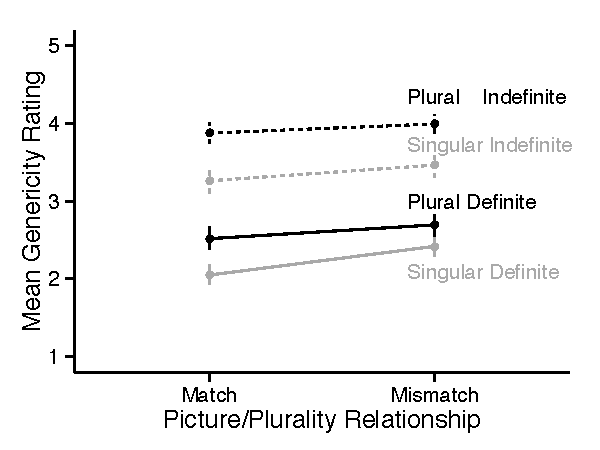
\includegraphics[width=.9\linewidth]{figures/e2b_mod.pdf}
\caption{\label{fig:e2b} Mean genericity ratings from Experiment 4 (independent ratings), plotted by picture/plurality match/mismatch, definiteness, and number. Error bars show 95\% confidence intervals.}
\end{figure}

Findings regarding subject NP types were largely comparable to Experiments 1. In addition, participants were more likely to interpret a sentence as generic when its subject NP failed to refer in context (Figure \ref{fig:e2b}). This effect was consistent across all NP types.

As in Experiment 1, we fit a linear mixed-effects model to predict participants' genericity ratings. We examined the interaction of animacy, definiteness, and number of the subject NP, as well as image match/mismatch.\footnote{The model specification was as follows: \texttt{response} \(\sim\) \texttt{animacy * definiteness * number * image + (animacy + definiteness + number + image | WorkerId) + (definiteness + number + image | subject noun)}.}. This model revealed main effects of definiteness, number, and image. Sentences with indefinite subject NPs were rated more generic (\(\beta = 1.40, t = 11.72,~p < 0.01\)), while sentences with singular subjects were rated less generic (\(\beta = -0.42, t = -3.64,~p < 0.01\)). Sentences appearing with an image that mismatched the subject NP in number were rated more generic (\(\beta = 0.38, t = 3.60,~p < 0.01\)). We also found interaction effects between between definiteness and image between animacy and image. Sentences with indefinite subjects that appeared with mismatching images were less generic (\(\beta = -0.30, t = -2.02,~p = 0.04\)), and sentences with inanimate subjects and mismatching images were less generic (\(\beta = -0.38,~t=-2.51,~p=0.01\)). Finally, the model showed a significant three-way interaction such that inanimate, indefinite subjects with mismatching images were rated significantly more generic (\(\beta = 0.43, t = 2.03,~p = 0.04\)).

These results are consistent with the prediction that contexts in which a referent is not available for the subject NP support generic interpretations. However, the effect size of this contextual manipulation was relatively small, especially compared to the effect of morphosyntactic factors. This leads us to believe that individuals are highly attuned to the role of morphosyntactic cues in conveying generic or non-generic meanings. Participants may have inferred from these morphosyntactic cues that there was some particular entity or event to which the sentence referred, even if this entity or event was not part of the immediate context.

\section{General Discussion}

We set out to explore the question of what gives rise to generic interpretations of sentences. Several of the results found here replicate previous findings about cues to genericity: Indefinites are more generic than definites \cite{Cimpian:2011, Gelman:2003}, animates are more generic than inanimates \cite{Brandone:2009}, and contextual factors influence generic interpretation \cite{Gelman:2003}. However, we have also established important generalizations about which factors are most important in driving generic interpretations. Definiteness and tense were shown to be incredibly important factors in driving generic interpretations in Experiments 1, 2, and 3. The results of Experiments 4 show that pragmatic cues regarding contextual referents also play a crucial role in allowing language users to identify generics. Importantly, although small, this effect was observed consistently all subject NP types.

Despite the diversity of factors that play a role in driving generic interpretations, many of these findings can be synthesized in the general claim that generic interpretations arise as the result of reference failure. This idea provides a straightforward explanation of the importance of definiteness of a sentence's subject NP and tense in guiding interpretations, as well as the effect of context revealed in Experiment 4.

\section{Acknowledgments}

Thanks to Daniel Lassiter, Rose Schneider, and the members of the Language and Cognition Lab. We gratefully acknowledge the support of ONR Grant N00014-13-1-0287.

\bibliographystyle{apacite}

\setlength{\bibleftmargin}{.125in}
\setlength{\bibindent}{-\bibleftmargin}

\bibliography{Generics}


\end{document}
